% =========================================================
% CHAPTER 4: SYSTEM ARCHITECTURE
% =========================================================

\chapter{SYSTEM ARCHITECTURE}
\label{chap:system_architecture}

QueryPilot is structured as a ten-component pipeline architecture. Each
component has a well-defined responsibility and communicates with adjacent
components through Python function calls and shared data structures. The
overall architecture is shown in \figref{fig:architecture}. This chapter
describes each component and its role within the system.

\begin{figure}[htbp]
  \centering
  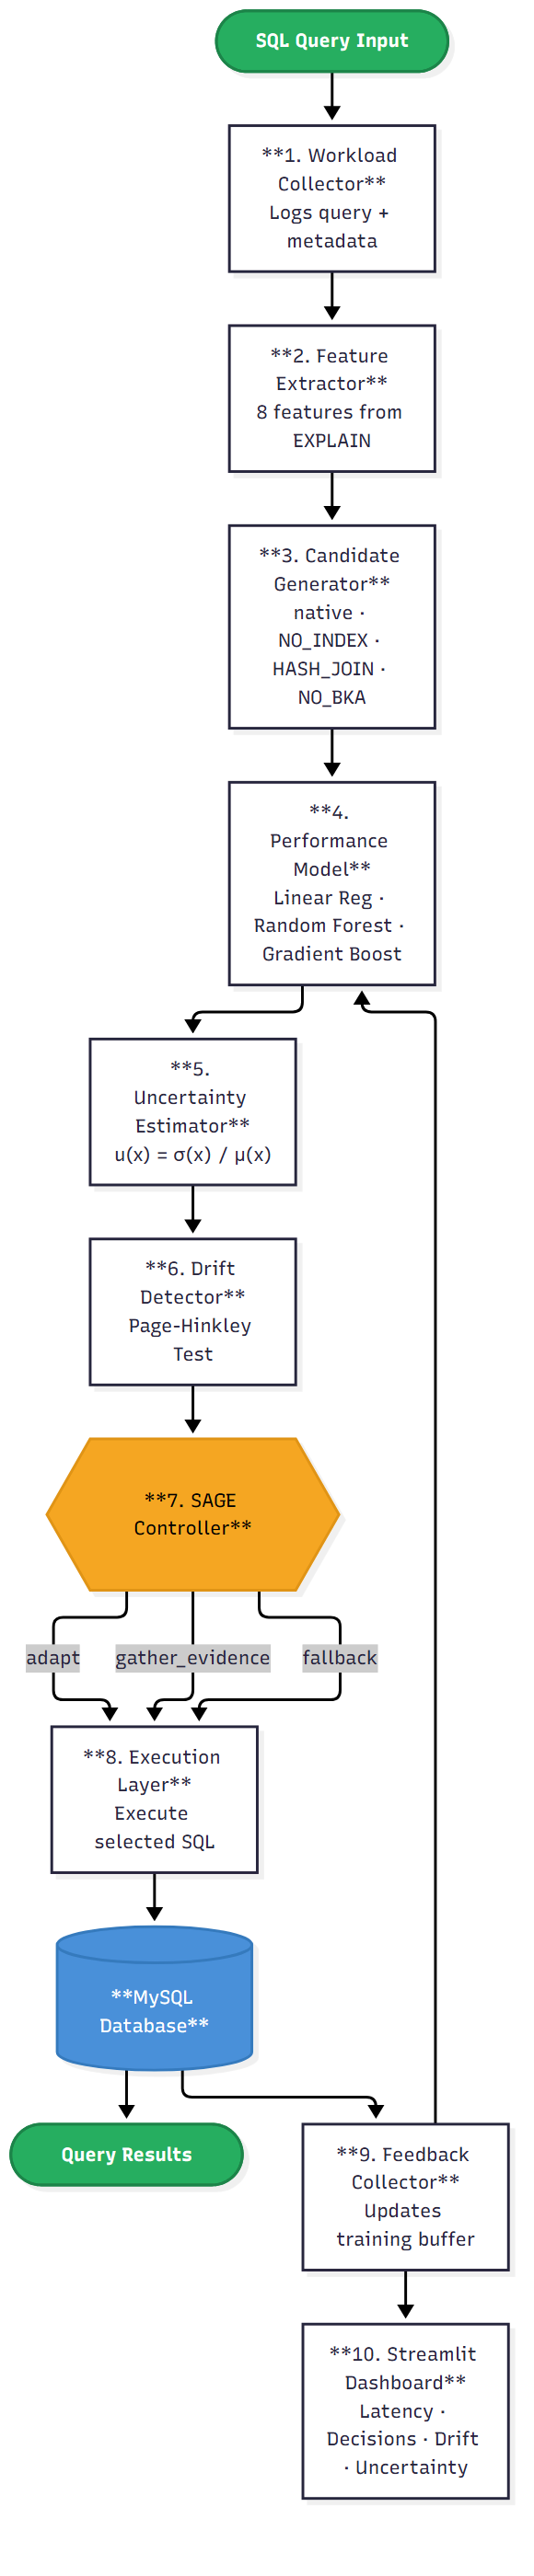
\includegraphics[width=0.95\textwidth]{figures/querypilot_arch}
  \caption{QueryPilot System Architecture: Ten-Component Pipeline}
  \label{fig:architecture}
\end{figure}

As depicted in \figref{fig:architecture}, the ten components form a directed
pipeline from query ingestion to result delivery. Each component is described
below.

\section{SYSTEM COMPONENTS}
\label{sec:system_components}

\textbf{MySQL Database.} The MySQL Database component stores the experimental
dataset and executes SQL queries. In this project, MySQL 8.0.43 is used with
the TPC-H benchmark loaded at scale factor 1, providing approximately 8.6
million rows across eight tables: region, nation, supplier, part, customer,
orders, partsupp, and lineitem. Standard indexes are applied to foreign key
columns and frequently filtered columns including order date, ship date, and
market segment. The database serves as the authoritative execution engine;
QueryPilot does not modify its internals in any way.

\textbf{Workload Collector.} The Workload Collector is the entry point of the
QueryPilot pipeline. It receives SQL queries from the application, records
arrival metadata, and forwards each query to the downstream components for
processing. In the current implementation, the collector is integrated into
the SAGEController's execute method, which intercepts queries before they
reach MySQL. The collector also maintains the count of queries seen, which
governs the gather-evidence phase.

\textbf{Feature Extractor.} The Feature Extractor derives a compact,
fixed-dimensional feature vector from each incoming SQL query. It runs
MySQL's EXPLAIN command on the query and parses the resulting execution plan.
Eight features are extracted: query type encoded as an integer, number of
explicit JOIN clauses, number of tables in the plan, boolean flags for
the presence of WHERE, GROUP BY, and ORDER BY clauses, the sum of estimated
rows across all plan rows, and a binary flag indicating whether any table
accesses use an index. These features form the input to the performance
prediction model.

\textbf{Candidate Optimization Generator.} The Candidate Generator produces a
controlled set of SQL variants by injecting MySQL optimizer hints into the
original query. The supported hint types are: native (the unmodified query),
NO\_INDEX (disables index usage on the first table in the plan), HASH\_JOIN
(forces a hash join between the first two joined tables, generated only for
queries with explicit JOIN clauses), and NO\_BKA (disables Batched Key Access
on the first table). A maximum of four candidates is generated per query.
The generator uses MySQL's EXPLAIN output to identify table names for hint
injection, ensuring that hints reference tables that actually appear in the
plan.

\textbf{ML Performance Prediction Model.} The Performance Prediction Model
estimates the expected execution time in milliseconds for each candidate
query. It maintains an ensemble of three scikit-learn models: a Linear
Regression, a Random Forest Regressor with 50 estimators, and a Gradient
Boosting Regressor with 50 estimators. The ensemble is trained on
(feature\_vector, execution\_time\_ms) pairs collected from previously
executed queries. The training buffer accumulates observations and triggers
a full retraining of all three models when it reaches the minimum evidence
threshold of ten observations. The ensemble mean serves as the point
prediction for each candidate.

\textbf{Uncertainty Estimator.} The Uncertainty Estimator computes the
relative disagreement among the three ensemble members as a proxy for
prediction confidence. For a given feature vector $x$, it computes
$u(x) = \sigma(x) / \mu(x)$, where $\mu(x)$ is the ensemble mean and
$\sigma(x)$ is the ensemble standard deviation. A higher value of $u(x)$
indicates that the three models disagree substantially about the expected
execution time, which signals that the prediction is unreliable. Candidates
with $u(x) > \tau_u = 0.8$ are excluded from SAGE's consideration.

\textbf{SAGE Decision Controller.} The SAGE (Stability-Aware Guarded
Execution) controller is the decision-making core of QueryPilot. It combines
the uncertainty estimates, the drift detector's state, and the performance
predictions to select one of three actions: gather evidence, fallback, or
adapt. The controller maintains the drift active flag, the training buffer,
the query counter, and the model instance. It enforces the regression
tolerance $\tau_r = 0.15$, ensuring that no candidate predicted to be more
than 15\% slower than native is ever selected.

\textbf{Query Execution Layer.} The Query Execution Layer issues the SQL
selected by SAGE to MySQL using the mysql-connector-python library. It
measures client-side execution latency using Python's time.perf\_counter()
function, which captures the elapsed time from the moment the SQL is sent to
MySQL until all results are fetched by the Python process. The measured time
includes network transfer and result serialization overhead in addition to
server-side query processing time.

\textbf{Feedback and Metrics Collector.} The Feedback Collector records the
outcome of each query execution. It appends the (feature vector, actual
execution time) pair to the training buffer for future model retraining. It
also updates the Page-Hinkley drift detector with the actual execution time.
Additionally, the MetricsLogger component appends a row to a CSV log file
recording the timestamp, query preview, SAGE decision, hint type selected,
execution time, prediction mean, prediction uncertainty, and drift detected
flag for every query. This log file is used by the dashboard for visualization.

\textbf{Streamlit Dashboard.} The Streamlit Dashboard provides a real-time
web-based visualization of QueryPilot's operation. It reads result JSON files
from the experiments directory and presents four pages: an Overview page
showing latency summary tables and bar charts, a Query Timeline page showing
per-query execution times for all three configurations with drift events
marked as red triangles, a SAGE Decisions page showing a pie chart of decision
type distribution and a table of recent decisions with their reasons, and an
Experiment Comparison page showing grouped bar charts across all scenarios.
